\documentclass[12pt,a4paper]{article}
% -- LuaLaTeX --
% !TEX root = ./main.tex
% !TEX program = lualatex

\usepackage{./tex/qdipsettings}
\usepackage{everypage}

\newcommand{\dadada}{%
  \begin{textblock*}{\textwidth}(30mm,20mm)
    \color{red}\transparent{0.2}
    \scalebox{7}{\rotatebox{60}{\framebox{НЕ ОПЛАЧЕНО}}}
  \end{textblock*}
}

%\AddEverypageHook{\dadada}

% настройки титульной страницы

\faculty{Институт \textnumero 4 -- Институт вычислительных систем и программирования}
\speciality{09.03.01}
\department{44}

\studclass{4241}
\studname{Гетманенко Г.В.}

\docfooter{Санкт-Петербург, 2016}

\docsubject{\uppercase{\large Текстовый редактор с шифрованием}}

%\nofiles

%\directlua{ require("drawboxes")}\usepackage{atbegshi}\AtBeginShipout {\directlua{drawboxes.visual_debug()}}

% нумерация рисунков по секциям
\counterwithin{figure}{section}

% ---------- НАЧАЛО ДОКУМЕНТА ----------

\begin{document}

% Титульник
\makeqdiptitle %
\qdipzad %
\newpage

\setcounter{page}{3}

% Содержание
\renewcommand{\contentsname}{{\centering\Large Содержание\par}}
\tableofcontents
% \addtocontents{toc}{\protect\thispagestyle{empty}} % убирает нумерацию в содержании
\newpage

% Сокращения
% !TEX root = ../main.tex
\newpage
\ssection{Список сокращений}

\noindent
GnuPG, GPG -- GNU Privacy Guard.\\
ECB -- Electronic Codebook (режим электронной кодовой книги , режим простой замены).\\
CBC -- Cipher Block Chaining (режим сцепления блоков шифротекста).\\
CFB -- Cipher Feedback (режим обратной связи по шифротексту).\\
OFB -- Output Feedback (режим обратной связи по выходу).\\
GPL -- GNU General Public License.\\
MPL -- Mozilla Public License.


% Введение
% !TEX root = ../main.tex
\newpage
\ssection{Введение}

На современном этапе развития IT-технологий имеются большие возможности
для несанкционированного доступа к хранимой информации. Существенную роль
играет вопрос о защите данных пользователя.

Для защиты данных от несанкционированного доступа используется множество
криптографических методов:
\begin{itemize}
    \item Симметричное шифрование;
    \item Асимметричное шифрование;
    \item Цифровые подписи;
    \item Хеширование.
\end{itemize}

Существует большое количество средств, использующих криптографические методы для
защиты данных пользователя, шифрования сообщений, подписания документов и т.д.

Сегодня у человека существует потребность в хранении большого объема конфиденциальной
информации. К этому понятию можно отнести персональные данные, телефонные номера,
контакты, пароли, личные заметки. Для решения этой задачи разрабатываются
пакеты прикладных программ, облачные сервисы и клиентские приложения.

Целью работы является проектирование и разработка программного средства
с графическим интерфейсом для создания, редактирования и просмотра
зашифрованных текстовых документов ``на лету''.

Для достижения этой цели были поставлены следующие задачи:
\begin{enumerate}
    \item Провести исследование и составить характеристику существующих
    пакетов и клиентских приложений, предоставляющих аналогичный функционал;
    \item На основании проведенного исследования и обзора определить
    задачи по разработке программного средства.
\end{enumerate}


% Основные разделы
% !TEX root = ../main.tex
\newpage
% Раздел 1
\section{Анализ предметной области}\label{sec:razd1}
% анализ предметной области

\subsection{Обзор аналогичных программ}
\label{ssec:obzor}

% --------------------------------------------------
\subsubsection{GNU Privacy Guard}

% http://citforum.ru/security/cryptography/gnupg/

GNU Privacy Guard (GnuPG, GPG) -- программа для шифрования
информации и создания электронных цифровых подписей \cite{gnupg}.
GNU Privacy Guard является продуктом с открытым кодом, созданным
сообществом разработчиков и распространяется под открытой лицензией General Public License (GPL).
Пакет изначально присутствует в любом дистрибутиве Linux и
используется во многих приложениях.

Основные функции GnuPG:
\begin{itemize}
    \item Шифрование текста и файлов (используется несколько алгоритмов);
    \item Подписывание документов электронной цифровой подписью и проверка чужих подписей;
    \item Создание и управление списками открытых ключей респондентов.
\end{itemize}

Следует отметить, что GnuPG является консольной утилитой, управляемой только из
командной строки. Для упрощения работы с GPG существуют несколько
графических оболочек а также множество компонент для разных языков.

В GnuPG используются разные криптографические алгоритмы: симметричные шифры,
шифрование с открытым ключом и смешанные алгоритмы.
Основной особенностью является система ключей. В GnuPG пользователь создает себе несколько
ключей, причем каждый служит для отдельного действия (и использует разные
алгоритмы). Длина ключа может быть в пределах от 1024 до 4096 бит.

Для работы с документами доступны несколько команд:
\begin{itemize}
    \item Подписать документ;
    \item Зашифровать документ;
    \item Подписать и зашифровать документ;
    \item Проверить подпись.
\end{itemize}

Для шифрования файлов GnuPG использует не чистый алгоритм с открытым
ключом, а смешанный -- для документа формируется уникальный сеансовый ключ,
который шифруется шифром с открытым ключом, текст документа шифруется
симметричным шифром на основе сеансового ключа. Получатель с помощью своего
секретного ключа расшифровывает сначала сеансовый ключ, а потом с его помощью
сам документ. Такая схема работает быстрее, чем шифрование с открытым ключом,
а по надежности (криптостойкости) равна надежности самого слабого
из алгоритмов.

Теоретически, это позволяет упростить задачу дешифровки -- вместо взлома
системы шифрования с открытым ключом надо взломать только симметричный шифр,
то есть подобрать сеансовый ключ. Но такой метод даст возможность расшифровать
только одно сообщение, ведь для каждого документа сеансовый ключ генерируется
отдельно. Для симметричного шифрования по умолчанию применяется алгоритм CAST5.

GPG является многофункциональным инструментом для шифрования.
Однако, он не обеспечивает возможность редактировать зашифрованные файлы без предварительной
расшифровки. Поэтому в дополнение к самому пакету необходимо иметь
оболочку, которая предоставляет такой функционал.

% --------------------------------------------------
% \newpage
\subsubsection{Vi/Vim}

% http://askubuntu.com/questions/436851/encrypting-text-editor
% https://github.com/vim/vim
% http://www.techrepublic.com/blog/it-security/vim-offers-strong-file-encryption-with-blowfish/

Vim -- улучшенная версия консольного текстового редактора Vi для
операционных систем семейства UNIX. Редактор имеет большое количество функций,
одной из которых является возможность работать с зашифрованными
текстовыми файлами. Для шифрования используется алгоритм Blowfish.

При создании файла можно указать флаг \texttt{-x}:

\begin{verbatim}
vim -x filename.txt
\end{verbatim}

После чего редактор просит пользователя ввести пароль:
\begin{verbatim}
Enter encryption key: *****
Enter same key again: *****
\end{verbatim}

Дальнейшая работа с зашифрованными файлами в редакторе vim ничем
не отличается от редактирования обычных текстовых файлов. Алгоритм
Blowfish является симметричным, поэтому при открытии файла необходимо
ввести тот же самый пароль.

Особенностью Vim является отсутствие необходимости сохранять
расшифрованную копию файла на жесткий диск перед его изменением.

Недостатком Vim является сложность использования и интерфейс, основанный на текстовых командах и
клавиатурных сокращениях, сильно отличающийся от интерфейса большинства современных графических программ.
На освоение этого редактора требуется значительное время.

% --------------------------------------------------
\newpage
\subsubsection{CryptoTE}

% http://askubuntu.com/questions/436851/encrypting-text-editor
% https://panthema.net/2009/cryptote/

CryptoTE -- текстовый редактор со встроенной функцией шифрования.
Данная программа позволяет создавать зашифрованные контейнеры,
которые могут содержать несколько файлов. Файлы могут быть как
текстовыми, так и бинарными (изображения, архивы и т. п.).

Программа позволяет редактировать текстовые файлы внутри контейнера
(рисунок \ref{fig:cryptote}), просматривать бинарные файлы
в шестнадцатиричном формате. Имеется возможность импортировать
и экспортировать файлы из контейнера.

CryptoTE по умолчанию использует симметричный алгоритм Serpent и
библиотеку zlib для сжатия данных. Имеется встроенный генератор
паролей.

\noindent
\begin{minipage}{\textwidth}
  \vspace{3.5mm}
  \centering
  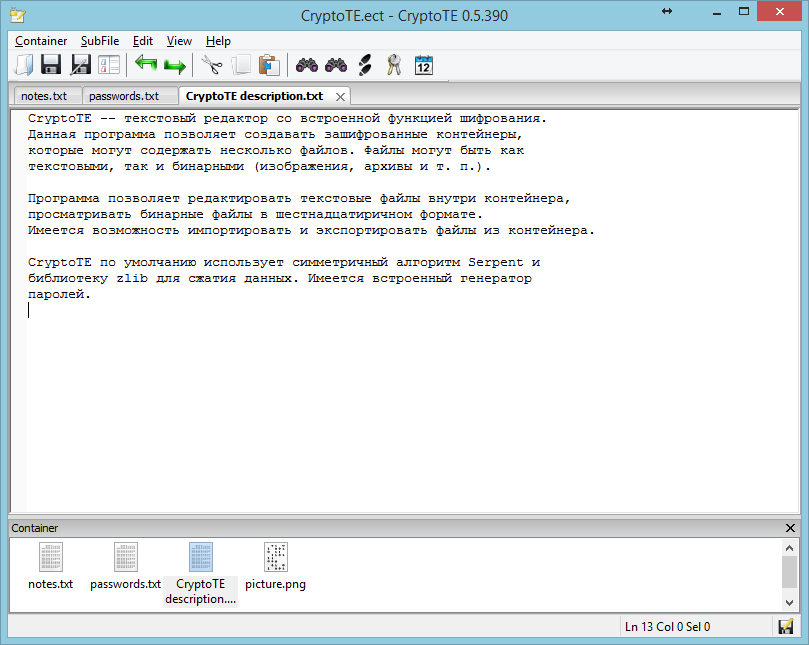
\includegraphics[scale=0.6]{./pics/cryptote-main.png}
  \captionof{figure}{Внешний вид редактора CryptoTE}\label{fig:cryptote}
  \vspace{3.5mm}
\end{minipage}

% --------------------------------------------------
\newpage
\subsubsection{KeyNote NF}

% http://jenyay.net/blog/2010/01/31/keynote-nf-eshhe-odin-outliner/

KeyNote NF -- структурный редактор (англ. outliner), позволяющий
структурированно хранить и редактировать заметки.

Файл с заметками может
содержать несколько вкладок, а каждая вкладка является
либо деревом заметок, либо одной заметкой с форматированием
(рисунок \ref{fig:keynotenf}). Сами заметки хранятся в формате
RTF (Rich Text Format). Программа позволяет шифровать файл
с заметками с помощью пароля.

\noindent
\begin{minipage}{\textwidth}
  \vspace{3.5mm}
  \centering
  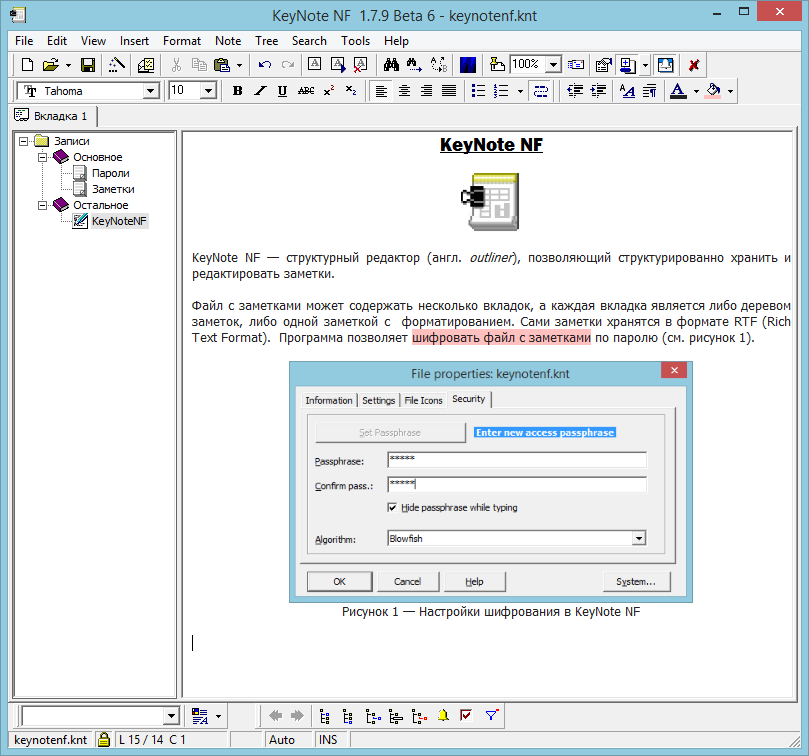
\includegraphics[scale=0.6]{./pics/keynote-main.png}
  \captionof{figure}{Внешний вид редактора KeyNote NF}\label{fig:keynotenf}
  \vspace{3.5mm}
\end{minipage}

% --------------------------------------------------
\newpage
\subsubsection{ProtectedText}

% https://www.protectedtext.com/
% https://play.google.com/store/apps/details?id=com.protectedtext.android

Приложение представляет из себя веб-сайт
\footnote{ProtectedText -- https://www.protectedtext.com/},
на котором любой пользователь имеет возможность бесплатно создать
одну или несколько страниц для хранения своих записей в текстовом
формате. Доступ к страницам осуществляется по паролю, который
вводит пользователь при первом сохранении текста на странице.
Страница может может содержать несколько вкладок
с текстовыми файлами (рисунок \ref{fig:protectedtext}).

По заверениям разработчиков, на сервере хранится только зашифрованный
текст и шифрование/дешифрование осуществляется на стороне пользователя.
С записками можно работать используя как персональный компьютер,
так и планшеты, смартфоны и остальные устройства с доступом в интернет.
При этом не требуется регистрация на сайте.

Стоит заметить, что пользователь может потерять доступ к своим записям
не только забыв пароль, но и потеряв ссылку на свою страницу с записями.

Пользователи устройств с ОС Anroid могут воспользоваться приложением
Safe Notes от разработчиков ProtectedText. Приложение позволяет создавать,
редактировать и шифровать заметки на мобильном устройстве, а так же
имеет возможность синхронизировать записи с ProtectedText.

\noindent
\begin{minipage}{\textwidth}
  \vspace{3.5mm}
  \centering
  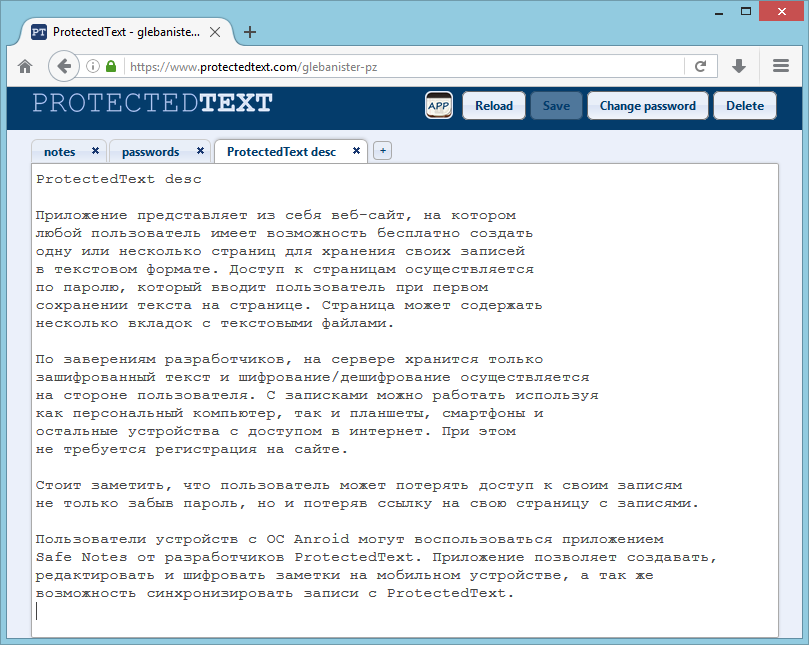
\includegraphics[scale=0.6]{./pics/protectedtext-main.png}
  \captionof{figure}{Внешний вид редактора ProtectedText}\label{fig:protectedtext}
  \vspace{3.5mm}
\end{minipage}

% --------------------------------------------------
\newpage
\subsubsection{NotepadCrypt}

% http://www.andromeda.com/people/ddyer/notepad/NotepadCrypt.html

NotepadCrypt -- простой текстовый редактор, основанный на Notepad2.
От Notepad2 редактор отличается наличием опции шифрования редактируемого
файла.

Приложение по умолчанию сохраняет текстовые файлы в незашифрованном виде.
Поэтому перед сохранением файла необходимо указать пароль, по которому
будет производиться шифрование (рисунок \ref{fig:notepadcrypt}).
Программа использует алгоритм шифрования AES-256.

Также стоит отметить возможность указать мастер-пароль (англ. master passphrase).
Файлы сохраненные с указанным мастер-паролем могут быть восстановлены
в случае утери пароля от зашифрованного файла.

\noindent
\begin{minipage}{\textwidth}
  \vspace{3.5mm}
  \centering
  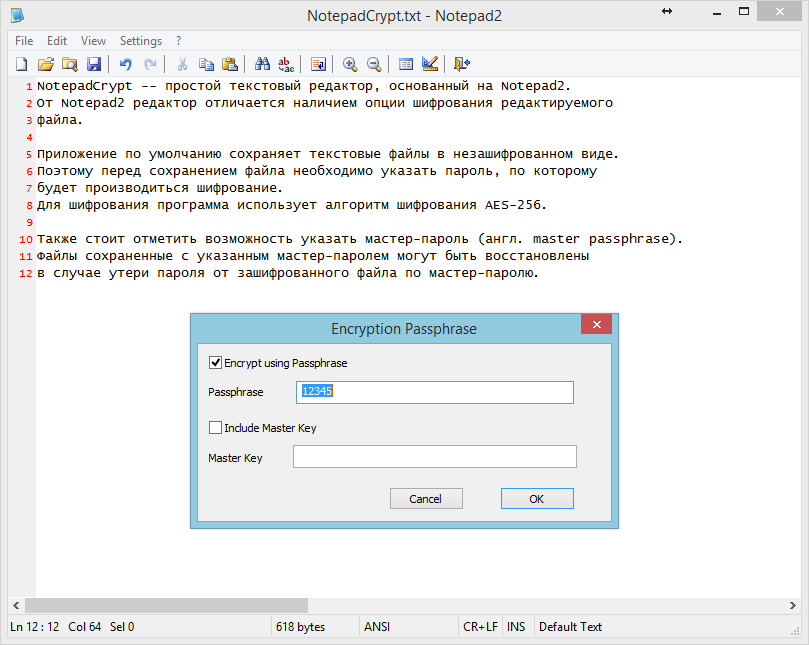
\includegraphics[scale=0.6]{./pics/notepadcrypt-main.png}
  \captionof{figure}{Внешний вид редактора NotepadCrypt}\label{fig:notepadcrypt}
  \vspace{3.5mm}
\end{minipage}

% --------------------------------------------------
\newpage
\subsubsection{Notepad++ (с аддоном NppCrypt)}

Notepad++ -- текстовый редактор, позволяющий расширить свой функционал
с помощью плагинов. Одним из интересных плагинов является NppCrypt.
Плагин дает возможность пользователю зашифровать текст.

В отличие от описаных ранее редакторов, плагин лишь изменяет выделенный
текст внутри редактора. Таким образом, перед сохранением отредактированного
текста пользователю необходимо его зашифровать, выбрав соответствующую опцию
в меню доступа к функциям плагина NppCrypt (рисунок \ref{fig:notepadpp}).
Аналогично после открытия зашифрованного файла необходимо выполнить
дешифрование, после чего можно приступить к редактированию текста.
Такая работа с файлом не слишком удобна и существенно снижает
эффективность пользователя.

В то же время плагин имеет довольно гибкие настройки и множество опций
симметричного шифрования. Шифротекст может храниться в бинарном,
в шестнадцатиричном виде или в кодировке base64. Текст можно зашифровать
одним из множества алгоритмов (IDEA, CAST5, Blowfish, AES-256 и т. д.).
Плагин позволяет выбрать один из нескольких режимов
шифрования (ECB, CBC, CFB, OFB и т. д.). Также имеются настройки
алгоритма генерации ключа по паролю.

\noindent
\begin{minipage}{\textwidth}
  \vspace{3.5mm}
  \centering
  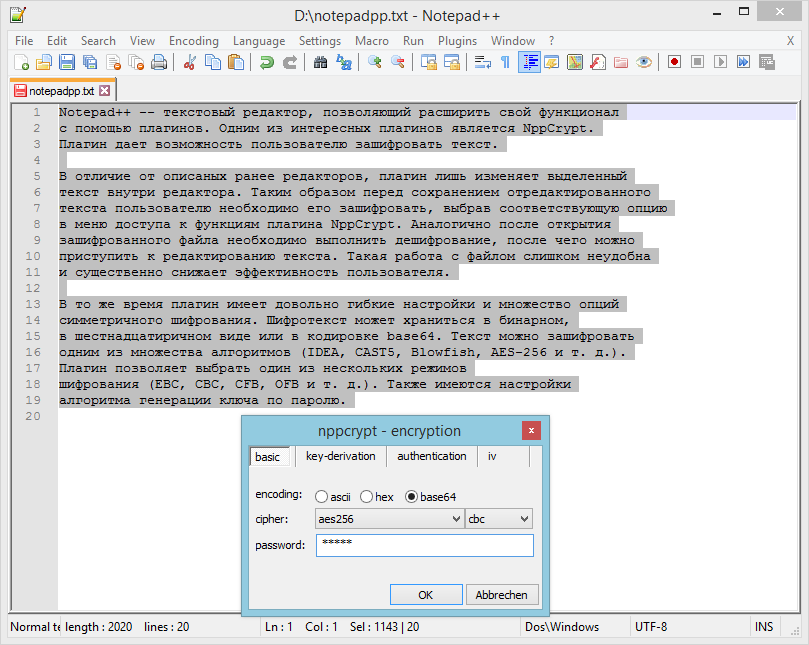
\includegraphics[scale=0.6]{./pics/notepadpp-main.png}
  \captionof{figure}{Внешний вид редактора Notepad++}\label{fig:notepadpp}
  \vspace{3.5mm}
\end{minipage}

% % --------------------------------------------------
% \subsubsection{Bitmask}
%
% Bitmask -- приложение с открытым исходным кодом, обеспечивающее легкую в
% использовании и безопасную зашифрованную коммуникацию.
% Bitmask предоставляет сервис для шифровании электронной почты, которая
% в то же время обратно совместима с существующим протоколом OpenPGP для
% безопасной электронной почты.
%
% В число особенностей программы входят:
% \begin{itemize}
%     \item Полное сквозное шифрование. Всякий раз, когда это возможно, все
%     сообщения шифруются непрерыно на клиентском устройстве.
%     \item Безопасное хранение. Все входящие сообщения автоматически шифруются,
%     потому только вы можете прочесть их (в том числе мета-данные).
%     \item Автоматическое управление ключами. Пользователю не нужно
%     беспокоиться о генерации, обнаружении или проверке ключей.
% \end{itemize}
%
% \subsubsection{opmsg}
%
% % https://github.com/stealth/opmsg
%
% Opmsg является альтернативой GPG для шифрования и подписания почтовых сообщений.
% Программа распространяется под лицензией GPLv3.


\newpage
\subsection{Сравнительный анализ}

В таблице \ref{tab:sravn} приведен сравнительный анализ описанных
в пункте \ref{ssec:obzor} программных средств для шифрования
текстовых документов.

\noindent
\begin{minipage}{\textwidth}
  \vspace{3.5mm}
  \captionof{table}{Сравнение приложений для шифрования текстовых записей}
  \vspace{-3.5mm}
  \label{tab:sravn}
  \footnotesize
  \begin{tabular}{|L{25mm}|L{30mm}|L{30mm}|L{40mm}|C{25mm}|}
    \hline
    Название &
      Лицензия &
      %Открытость кода &
      Операционная система &
      Криптографические методы &
    Графический интерфейс \\\hline

    GNU Privacy Guard &
      GNU GPLv3 &
      %Код открыт &
      Linux, Windows, Mac OS X &
      AES, DES, Blowfish, CAST5, MD5, SHA1, SHA256, SHA512, RSA, ... &
      $-$
    \\\hline

    Vim  &
      GPL-совместимая &
      %Код открыт &
      Linux, Windows, OS X &
      Blowfish &
      $-$
    \\\hline


    CryptoTE &
      GNU GPLv2 &
      %Код открыт &
      Linux, Windows &
      Serpent &
      $+$
    \\\hline

    KeyNote NF &
      MPLv2.0 &
      %Код открыт &
      Windows &
      Blowfish, IDEA &
      $+$
    \\\hline


    ProtectedText &
      \makebox[30mm][c]{$-$} &
      %Частично открыт &
      Веб-приложение &
      AES, SHA256 &
      $+$
    \\\hline

    NotepadCrypt &
      GNU GPLv3 &
      %Код открыт &
      Windows &
      AES, SHA256 &
      $+$
    \\\hline

    Notepad++ (NppCrypt) &
      GNU GPLv3 &
      %Код открыт &
      Linux, Windows &
      AES, DES, CAST5, IDEA, Blowfish,
      MD5, SHA1, SHA256, SHA512, ... &
      $+$
    \\\hline
  \end{tabular}
  \vspace{3.5mm}
\end{minipage}

\subsection{Постановка задачи}
Безопасное хранение и быстрый доступ к конфиденциальной информации -- важная
задача для современного пользователя. При этом немалое значение имеет простота интерфейса:
многие эффективные средства защиты информации оказываются недоступными для большинства пользователей из-за
сложности освоения. Сравнительный анализ показывает, что
актуально и целесообразно спроектировать и реализовать программный продукт
в соответствии со следующими требованиями:
\begin{itemize}
    \item Наличие графического интерфейса;
    \item Работа с зашифрованными файлами с использованием прозрачного шифрования;
    \item Поддержка различных алгоритмов шифрования;
    \item Мультиплатформенность.
\end{itemize}

% !TEX root = ../main.tex
\newpage
% Раздел 2
\section{Теоретические сведения}\label{sec:razd2} % Теоретические сведения

\subsection{Языки программирования и библиотеки}

В качестве основного языка был выбран Python -- высокоуровневый интерпретируемый
язык программирования общего назначения с динамической типизацией
данных \cite{python}.

К достоинствам Python можно отнести:
\begin{itemize}
    \item Язык является интерпретируемым (не требует компиляции), что повышает
    производительность разработчика при написании и отладке программного кода.
    \item Кроссплатформенность. Основной интерпретатор языка (CPython)
    реализован для большинства активно используемых платформ, что позволяет
    использовать один и тот же код на любой системе.
    \item Имеется большая стандартная библиотека и множество пользовательских
    модулей, находящихся в открытом доступе.
\end{itemize}

Основные недостатки языка:
\begin{itemize}
    \item Низкое быстродействие;
    \item Не слишком удачная поддержка многопоточности.
\end{itemize}

Реализуемая программа состоит из двух частей:
\begin{enumerate}
    \item Графический интерфейс;
    \item Подсистема шифрования.
\end{enumerate}

Графический интерфейс программы был реализован с использованием библиотеки Qt5
и ее привязки к Python -- PyQt5.

Несмотря на особенности выполняемой задачи (шифрование текстовых документов),
в общем случае шифрование должно выполняться эффективно по времени.
Из-за низкой скорости выполнения кода использовать Python для реализации криптографических
методов, в частности алгоритмов шифрования, является нежелательным.
Для повышения производительности рассмотрено две альтернативы: использовать язык C (стандарт C99) или
язык ассемблера. В разделе \ref{sec:razd3} приведен краткий анализ реализаций
алгоритмов шифрования на языке ассемблера и C.

\newpage
\subsection{Алгоритмы шифрования}

В проекте на данный момент реализовано два алгоритма шифрования:
FEAL-4 и Blowfish. Выбор первого обусловлен простотой реализации и
довольно высокой скоростью работы, несмотря на невысокую криптографическую
стойкость: шифр может быть взломан по пяти подобранным исходным блокам
с использованием линейного криптоанализа \cite{feal-attack}.

Алгоритм Blowfish является безопасным незапатентованным свободным для
использования шифром. На данный момент, в отличие от FEAL-4, не существует
эффективных методов взлома шифра Blowfish.

Алгоритм FEAL (Fast data Encipherment ALgorithm) был разработан криптографами
Акихиро Симидзу (Akihiro Shimizu) и Сёдзи Миягути (Shoji Miyaguchi) из
японской компании NTT в 1987 г. \cite[стр. 206]{panasenko}.

Разработчики алгоритма продвигали FEAL как потенциальную замену стандарта
шифрования DES -- по их мнению, FEAL-4 (число в названии обозначает количество
раундов алгоритма) предлагал более быстрое шифрование без потери его качества.
Кроме того, в FEAL отсутствуют табличные замены, поэтому реализация алгоритма
не требует дополнительной энергонезависимой памяти для хранения таблиц.

На рисунке \ref{fig:feal-nx-structure} представлена структура общего варианта
алгоритма FEAL -- FEAL-NX -- вместе с функцией расширения ключа. В упрощенном
варианте алгоритма FEAL-4 функция расширения не используется, поэтому рассмотрена
не будет.

Алгоритм FEAL-4 имеет структуру сети Фейстеля:
в каждом раунде выполняется обработка правого 32-битного подблока функцией
$F(R,k_{16})$, где $R$ -- правый подблок данных, $k_{16}$ -- 16-битное значение
ключа раунда. Результат обработки накладывается на левой подблок операцией XOR.
Перед первым раундом выполняется операция $XOR$ блока шифруемых данных с
ключом, а также аналогичное наложение левого подблока на правый.
После финального раунда алгоритма также производятся те же действия:
наложение левого блока на правый и сложение с ключом.
Расшифрование выполняется аналогично, но 16-битовые подключи подставляются
в обратном порядке.

\noindent
\begin{minipage}{\linewidth}
  \centering
  \vspace{3.5mm}
  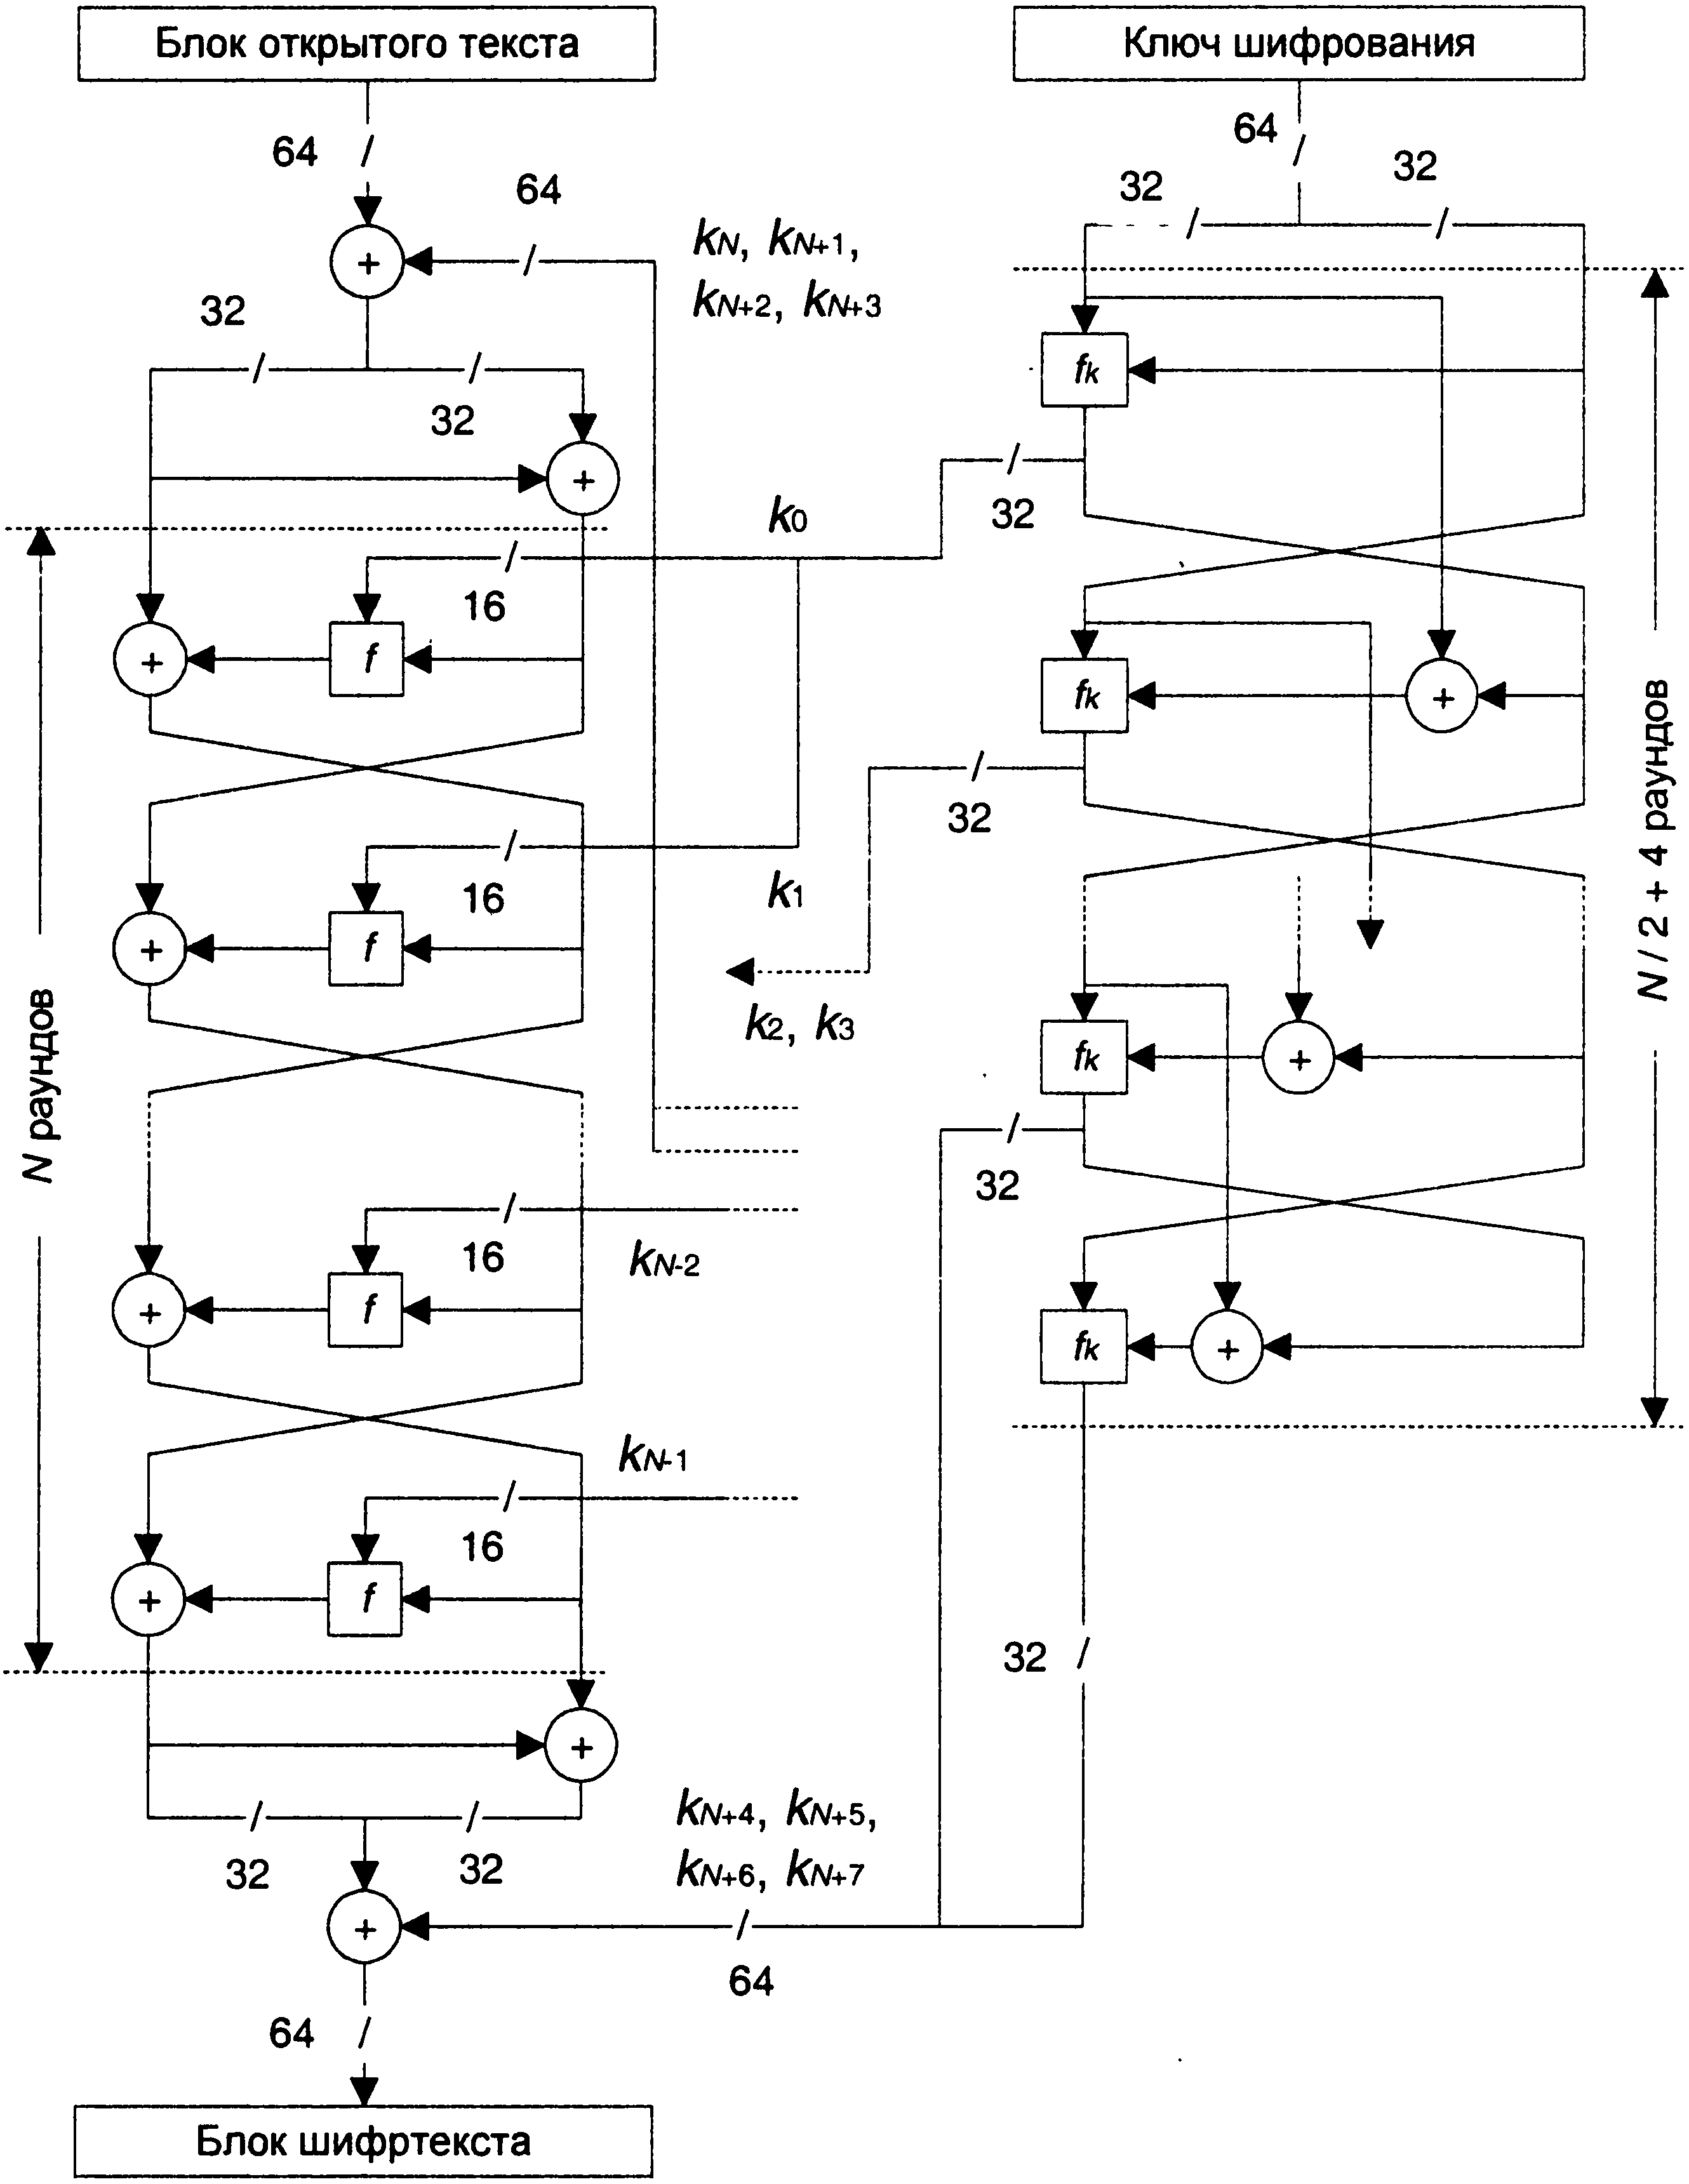
\includegraphics[scale=0.2]{./pics/feal-nx-structure.png}
  \captionof{figure}{Структура алгоритма FEAL-NX.}\label{fig:feal-nx-structure}
  \vspace{3.5mm}
\end{minipage}

Структура функции $F$ представлена на рисунке \ref{fig:feal-nx-f}.
В ней используются лишь три вида преобразований: операция $XOR$,
функции $S_0$ и $S_1$, которые можно описать следующим образом:
\begin{align*}
  S_0 = & \text{ROL}_2((x+y)\text{mod}2^8), \\
  S_1 = & \text{ROL}_2((x+y+1)\text{mod}2^8),
\end{align*}
где $\text{ROL}_2$ -- операция циклического сдвига влево на два разряда.

\noindent
\begin{minipage}{\linewidth}
  \centering
  \vspace{3.5mm}
  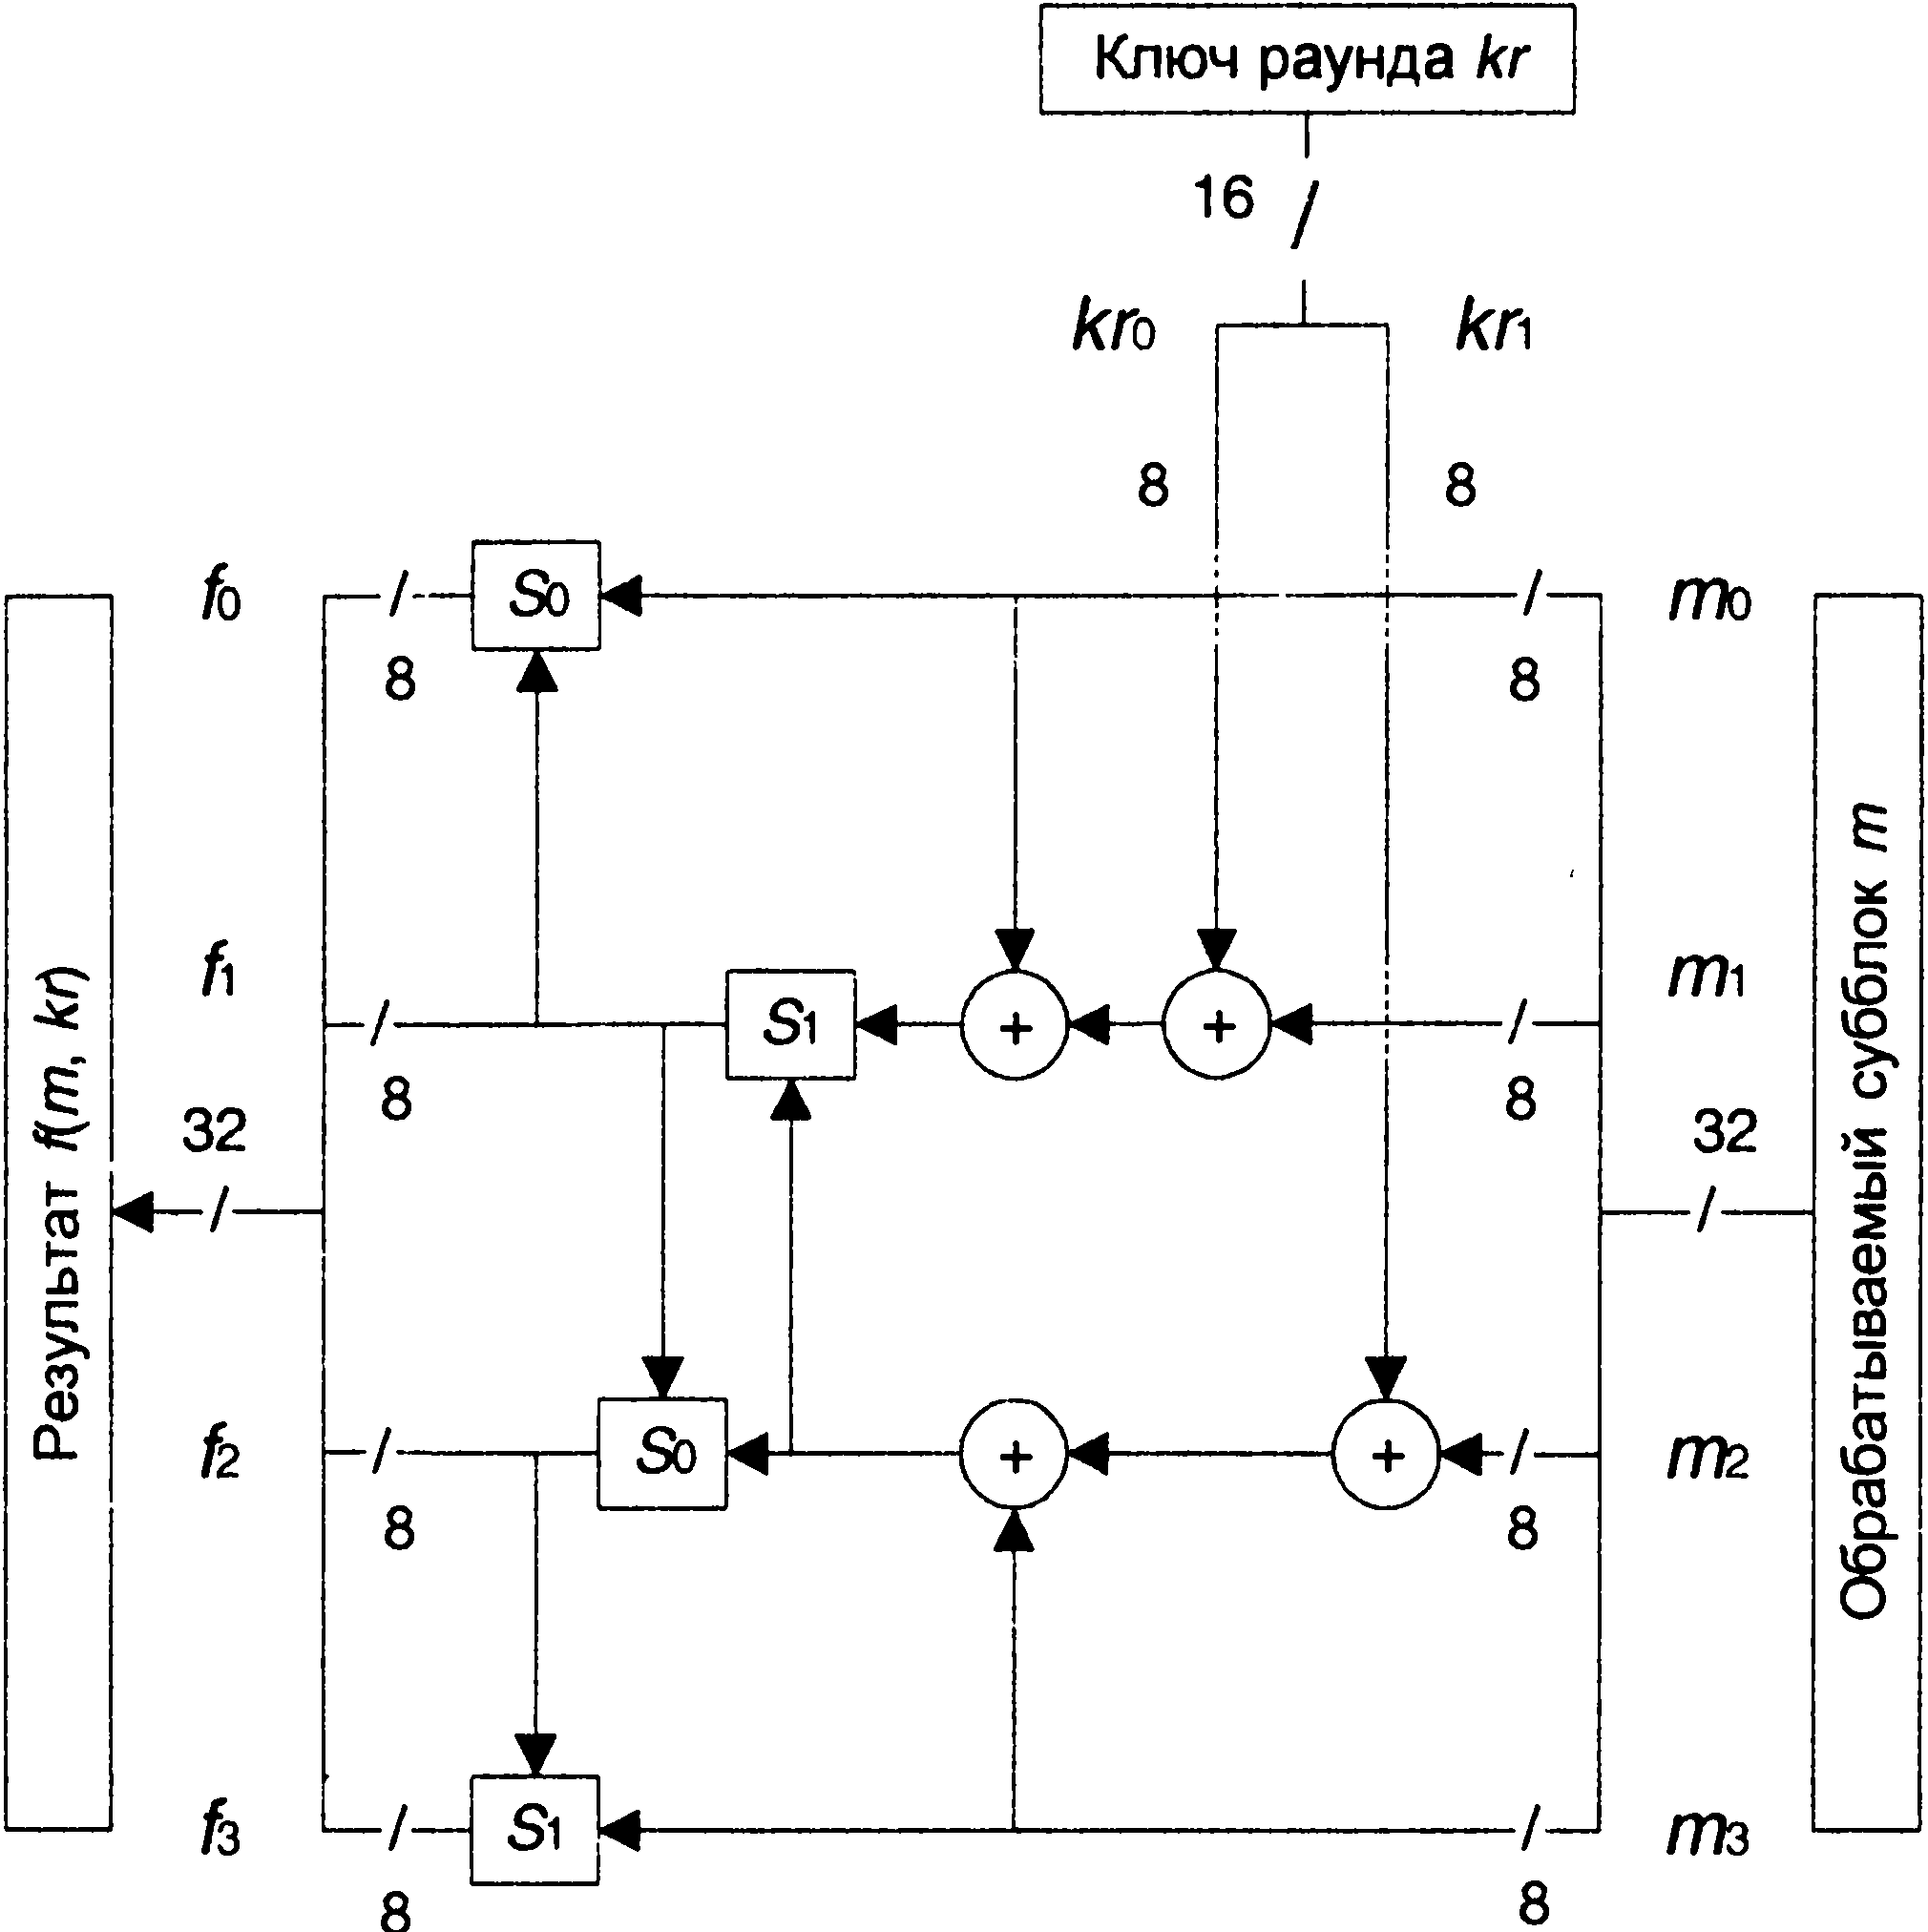
\includegraphics[scale=0.2]{./pics/feal-nx-f.png}
  \captionof{figure}{Функция $F$ алгоритма FEAL-4.}\label{fig:feal-nx-f}
  \vspace{3.5mm}
\end{minipage}

Алгоритм FEAL-4, изначально предлагавшийся в качестве замены стандарта DES,
оказался весьма нестоек к различным видам криптоанализа. Та же участь постигла
и алгоритм FEAL-8. Алгоритмы FEAL-16, FEAL-32 и т. д. оказались существенно
более стойкими за счет большего количества раундов. Однако скорость их работы
оказалась ниже скорости алгоритма DES. Поэтому, как стандарт шифрования,
алгоритм FEAL не состоялся.

Алгоритм Blowfish разработан Брюсом Шнайером в 1994 г. также в качестве
замены DES \cite[стр. 118]{panasenko}.
Алгоритм оказался весьма удачным и приобрел широкую популярность. Он очень широко реализован в различных
средствах защиты информации.

Blowfish, как и FEAL-4, шифрует данные 64-битными блоками, однако размер
ключа может варьироваться от 32 до 448 бит. Алгоритм также представляет
собой сеть Фейстеля, его структура приведена на рисунке \ref{fig:blowfish-structure}.

\noindent
\begin{minipage}{\linewidth}
  \centering
  \vspace{3.5mm}
  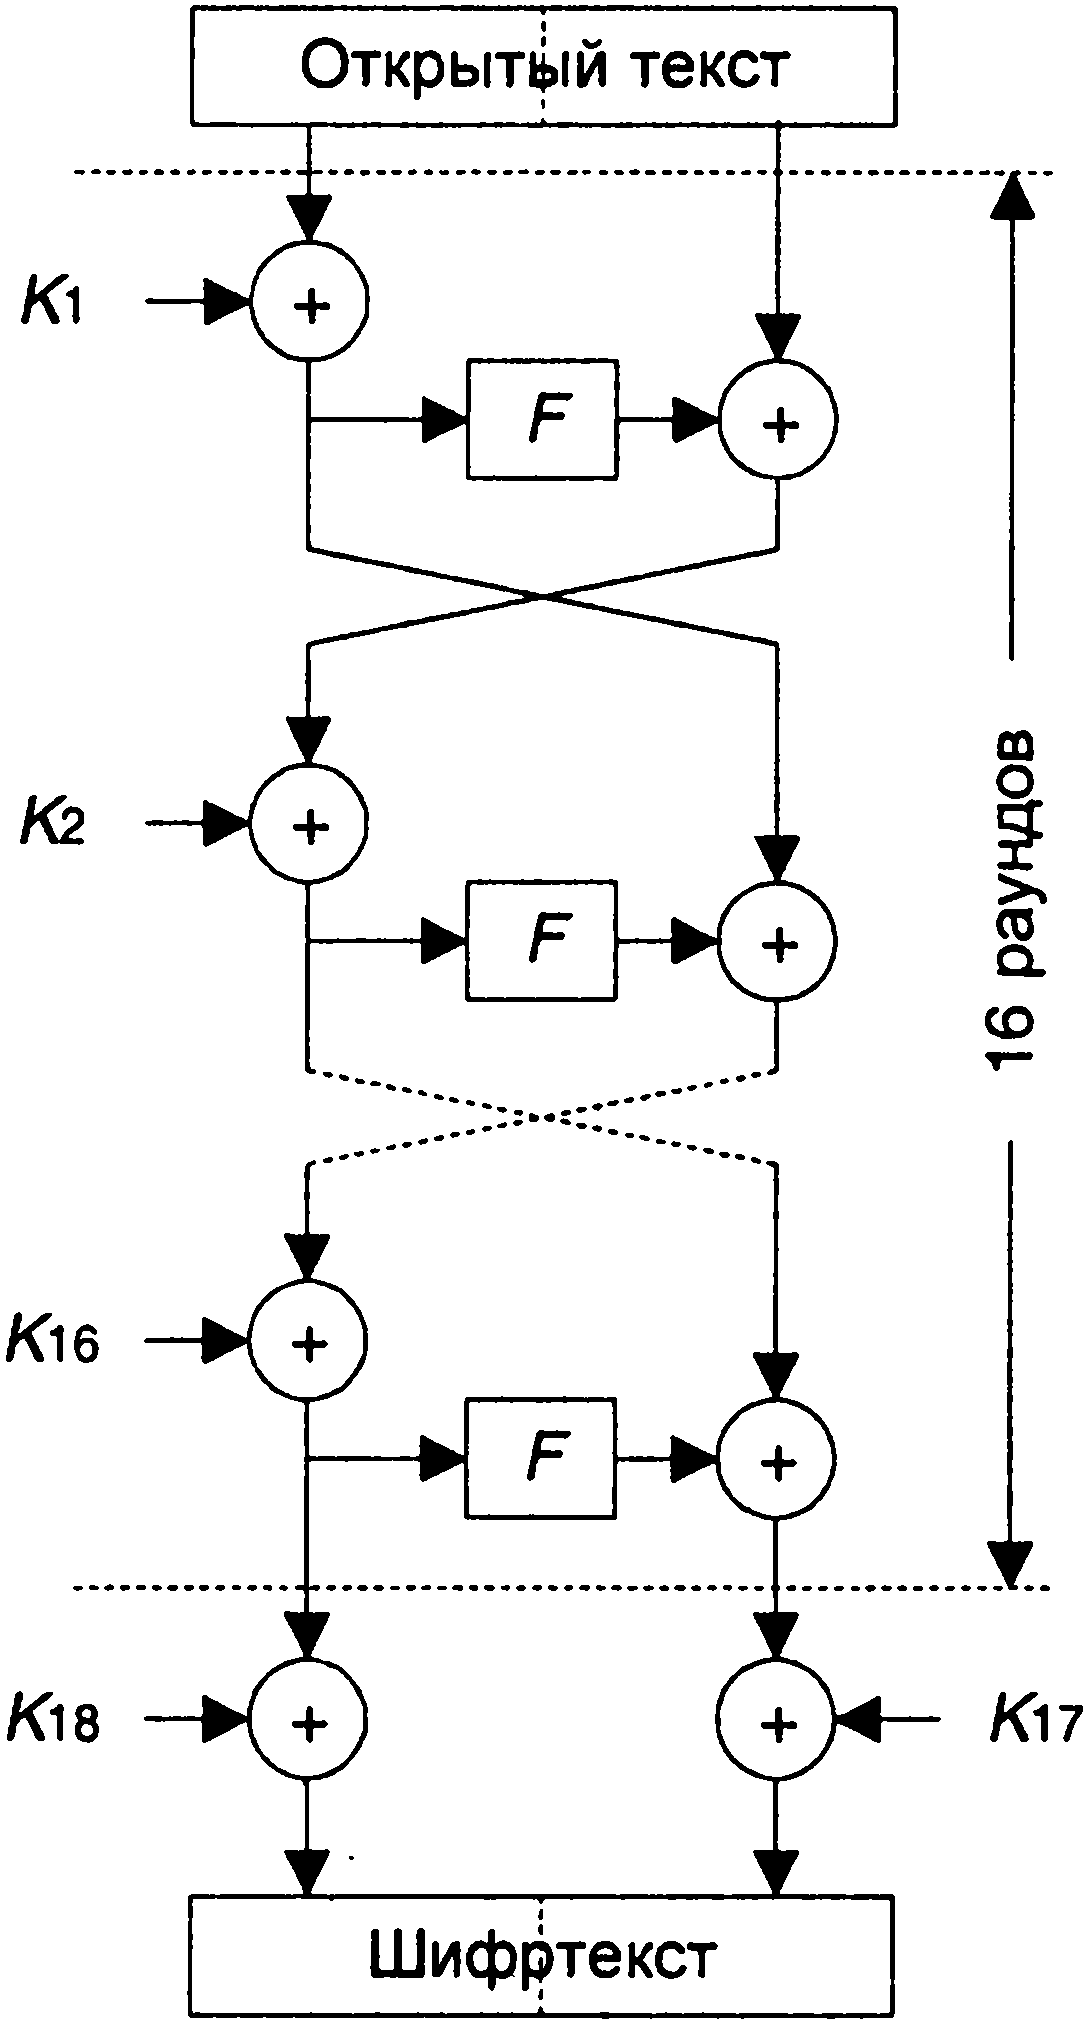
\includegraphics[scale=0.2]{./pics/blowfish-structure.png}
  \captionof{figure}{Структура алгоритма Blowfish.}\label{fig:blowfish-structure}
  \vspace{3.5mm}
\end{minipage}

Шифрование данных выполняется в 16 раундов, в каждом из которых над левым
32-битным подблоком данных производятся следующие действия \cite{blowfish}:
\begin{enumerate}
  \item Значение подблока складывается с ключом i-го раунда $K_i$ операцией
  $XOR$, результат операции становится новым значением подблока.
  \item Подблок обрабатывается функцией $F$. Результат обработки накладывается
  на правый подблок операцией $XOR$.
  \item Подблоки меняются местами во всех раундах, кроме последнего.
\end{enumerate}

После 16 раундов выполняется наложение на подблоки еще двух подключей:
$K_{17}$ и $K_{18}$ складываются операцией $XOR$ с правым и левым
подблоками соответственно.

Функция $F$ (рисунок \ref{fig:blowfish-f}) обрабатывает подблок следующим образом:
\begin{enumerate}
  \item 32-битное входное значение делится на четыре фрагмента по восемь битов,
  каждый из которых является индексом соответствующих таблиц замен $S_1..S_4$.
  \item Значения из таблиц $S_1$ и $S_2$ складываются по модулю $2^{32}$.
  \item Полученное значение складывается операцией $XOR$ со значением из $S_3$.
  \item Полученное значение складывается по модулю $2^{32}$ со значением из $S_4$.
\end{enumerate}

Расшифрование выполняется аналогично шифрованию, но ключи $K_1..K_{18}$
используются в обратном порядке.

\noindent
\begin{minipage}{\linewidth}
  \centering
  \vspace{3.5mm}
  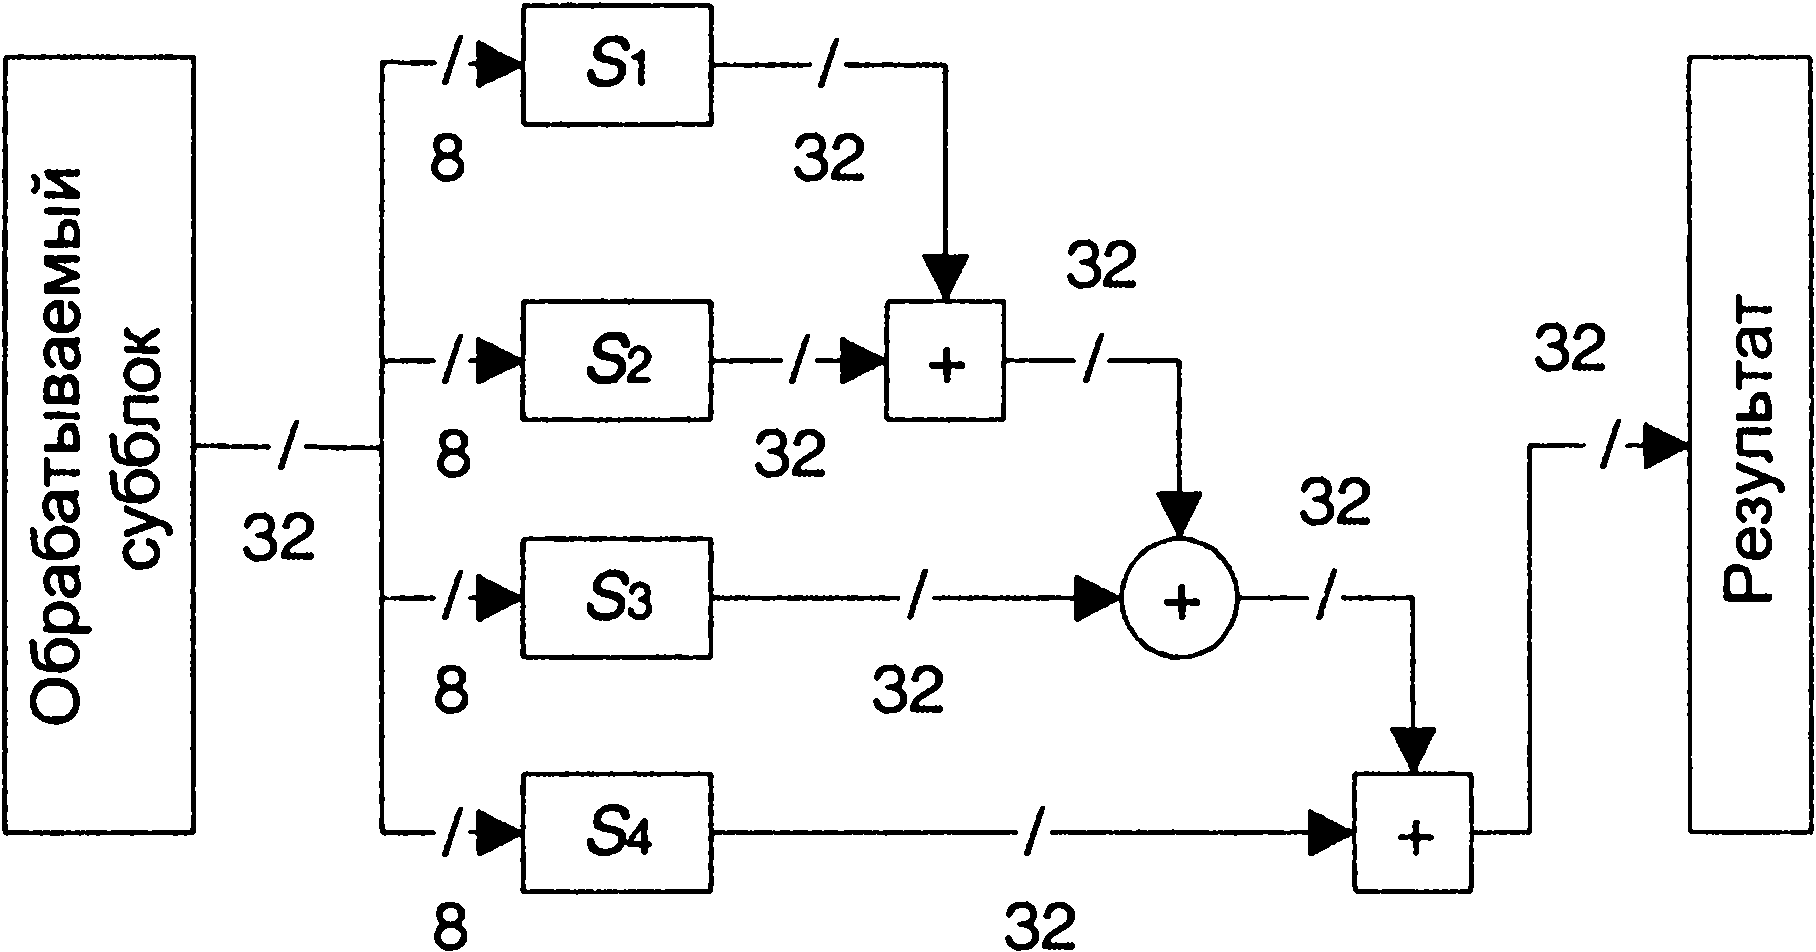
\includegraphics[scale=0.2]{./pics/blowfish-f.png}
  \captionof{figure}{Функция $F$ алгоритма Blowfish.}\label{fig:blowfish-f}
  \vspace{3.5mm}
\end{minipage}

В отличие от FEAL-4, перед шифрованием алгоритмом Blowfish необходимо
сгенерировать раундовые 32-битные ключи $K_1..K_{18}$ и четыре таблицы
замены $S_1..S_4$. Каждая таблица замены содержит 256 32-битных значений.

Процедура расширения ключа состоит из следующих шагов:
\begin{enumerate}
  \item Исходные значения ключей раундов и табилиц замен инициализируются
  псевдослучайно строкой, в качестве которой используется шестнадцатеричная
  запись дробной части числа $\pi$. Исходные значения ключей и таблиц можно
  найти в приложении В.
  \item Операцией $XOR$ на $K_1$ накладываются первые 32-бита ключа шифрования,
  на $K_2$ -- следующие 32 бита и т.д. до $K_{18}$. Ключ шифрования накладывается
  циклически, если используется более короткий ключ шифрования, чем необходимо
  для наложения на $K_1$..$K_{18}$.
  \item С использованием полученных ключей раундом и таблиц замен выполняется
  шифрование алгоритмом Blowfish блока данных, состоящего из 64 нулевых битов.
  Результат становится новым значением ключей $K_1$ и $K_2$.
  \item Используя измененные значения ключей $K_1$ и $K_2$, шифруется результат,
  полученный на предыдущем этапе. В результате получаются новые значения ключей
  $K_3$ и $K_4$.
  \item Шифрование выполняется до тех пор, пока новыми значениями не будут
  заполнены все ключи раундов и таблицы замен.
\end{enumerate}

Особенностью алгоритма Blowfish является то, что он не годится
для применения в случаях, где требуется частая смена ключей. Процедура
расширения ключа является достаточно ресурсоемкой, поэтому одно из достоинств
алгоритма Blowfish -- достаточно высокая скорость шифрования -- проявляется
только в тех случаях, если на одном ключе шифруется достаточно большой объем
информации. И наоборот, если менять ключ после каждого из шифруемых блоков,
скорость алгоритма становится катастрофически низкой именно из-за необходимости
каждый раз выполнять расширения ключа.

Явные достоинства и отсутствие критичных недостатков предопределили
широкое использование алгоритма Blowfish.

\subsection{Хранение данных}

Для хранения зашифрованных данных необходимо обеспечить:
\begin{itemize}
    \item Целостность данных;
    \item Поддержка нескольких алгоритмов шифрования и хэширования;
\end{itemize}

Для хранения зашифрованных данных была спроектирована структура файла,
включающая в себя:
\begin{enumerate}
  \item Заголовок.
  \begin{enumerate}
    \item Магическое число (сигнатура) -- 4 байта : \verb"'tfe', 0x42".
    \item Используемый алгоритм -- 1 байт.
    \item Используемая функция хэширования -- 1 байт.
    \item Отступ до зашифрованных данных от начала заголовка -- 2 байта.
    \item Размер исходных зашифрованных данных -- 8 байт.
  \end{enumerate}
  \item Преамбула.
  \begin{enumerate}
    \item Хэш первых 512 байт исходных данных -- размер зависит от
    используемой функции хэширования.
    \item Соль для пароля -- 16 байт.
  \end{enumerate}
  \item Зашифрованные данные.
\end{enumerate}

Используемый алгоритм и функция хэширования являются номерами
в таблицах функций алгоритмов и функций хэширования. На данный
момент реализована поддержка следующих функций:
\begin{itemize}
  \item Функции шифрования:
  \begin{enumerate}
    \item FEAL-4;
    \item Blowfish;
  \end{enumerate}
  \item Функции хэширования:
  \begin{enumerate}
    \item MD5;
  \end{enumerate}
\end{itemize}

При использовании блочного шифра в режиме EBC необходимо дополнить исходные
данные, чтобы их размер стал кратен размеру блока. В реализации последний
блок данных дополняется необходимым количеством байтов со значением 0x42.
При дешифровании лишние байты отрезаются, так как известен размер
зашифрованных данных.

Формат позовляет хранить зашифрованные данные любого типа,
есть возможность проверить полученные после расшифрования данные
на соответствие исходным данным (то есть проверить был ли использован
правильный ключ при расшифровании).

Однако такой формат может быть контейнером только для одного файла.
Отсутствует встроенная поддержка сжатия данных и возможность восстановить
тип исходного файла.

Несмотря на перечисленные ограничения, спроектированный формат зашифрованного файла
подойдет для использования в разрабатываемом программном средстве.

\subsection{Проектирование интерфейса}

Графический пользовательский интерфейс программы должен выглядеть
как обычный текстовый редактор (рисунок \ref{fig:generic-text-editor}).
В рамках рассматриваемой задачи интерфейс должен предоставлять
пользователю следующие функции:
\begin{itemize}
    \item Редактирование текстовых файлов;
    \item Шифрование текстовых файлов;
    \item Базовые настройки текстового редактора (внешний вид, шрифт);
    \item Основные настройки шифрования.
\end{itemize}

\noindent
\begin{minipage}{\linewidth}
  \centering
  \vspace{3.5mm}
  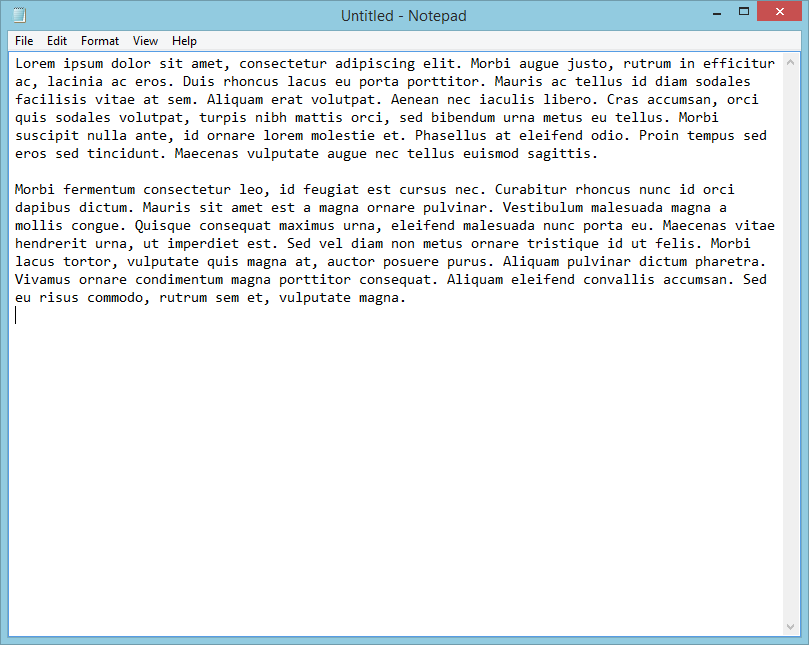
\includegraphics[scale=0.6]{./pics/generic-text-editor.png}
  \captionof{figure}{Интерфейс обычного текстового редактора.}\label{fig:generic-text-editor}
  \vspace{3.5mm}
\end{minipage}

% !TEX root = ../main.tex
\newpage
% Раздел 3
\section{Реализация}\label{sec:razd3}

% \subsection{Технология реализации} % ?
% ООП
% выбор языков программирования
% используемые библиотеки/модули
% git
%% работа с репозиторием
%% commitы

\subsection{Общее описание проекта} % ?
% Общее описание разработанного проекта
% Общее описание структуры проекта

Согласно поставленным задачам, проект должен содержать:
\begin{itemize}
  \item Реализацию алгоритмов шифрования;
  \item Модуль для работы с зашифрованными файлами;
  \item Описание пользовательского интерфейса;
  \item Файлы локализаций.
\end{itemize}

Для удобного взаимодействия разработчика с проектом,
была использована система контроля версий Git.
Структура репозитория была определена следующим образом:

\verbatiminput{./cont/app-raw-tree-desc.txt}

\emph{Алгоритмы шифрования} подключаются к программе как динамические
библиотеки. Реализация каждого алгоритма шифрования содержится в своей
директории отдельно от остальных исходников.

\emph{Модули программы} поделены на несколько частей:
\begin{itemize}
    \item Привязка динамических библиотек с алгоритмами шифрования к Python;
    \item Модуль для работы с разработанным форматом файла;
    \item Описание логики работы графического пользовательского интерфейса.
\end{itemize}

\emph{Файлы локализаций} содержат перевод строк, используемых в приложении:
`Файл', `правка', `сохранить', `копировать', `вставить' и т. д.

% сюда бы водички

Весь исходный код проекта содержится в репозитории на GitHub.
Веб-адрес репозитория: \verb'http://github.com/MrP4p3r/PyTFE'.

\newpage
Далее представлено содержание проекта на финальной стадии разработки:

\verbatiminput{./cont/app-tree.txt}

\newpage
\subsection{Реализация алгоритмов шифрования} % ?

Существуют различные режимы шифрования исходного текста блочным
шифром: режим простой замены (ECB), режим сцепления блоков (CBC),
режим обратной связи по шифротексту (CFB), режим обратной связи по
выходу (OFB) и др. Несмотря на явные недостатки режима ECB,
из-за простоты реализации был выбран именно он.

При выполнении работы были написаны реализации алгоритмов шифрования
FEAL-4 и Blowfish на языке ассемблера и на языке высокого уровня C.
Исходный код всех реализаций представлен в приложении А.

Для компиляции исходного кода на языке C был использован компилятор
GNU C Compiler (\texttt{gcc}),
для компиляции ассемблерного кода -- Flat Assembler (\texttt{fasm}).
Был проведен анализ скорости шифрования каждой из реализаций. Результаты
приведены в таблице \ref{tab:enc-speed-rez}.

\noindent
\begin{minipage}{\linewidth}
  \vspace{2.5mm}
  \captionof{table}{Результаты сравнения скорости работы алгоритмов}\label{tab:enc-speed-rez}
  \vspace{-2.5mm}
  \begin{tabular}{|l|l|l|l|}
    \hline
    Шифр            & Скорость шифрования/дешифрования \\\hline
    Blowfish (C)    & 151.7 Мб/с  \\\hline
    Blowfish (ASM)  & 108.4 Мб/с  \\\hline
    FEAL-4 (C)      & 234.3 Мб/с  \\\hline
    FEAL-4 (ASM)    & 382.4 Мб/с  \\\hline
  \end{tabular}
  \vspace{2.5mm}
\end{minipage}\\

Скорость выполнения кода на языке C зависит от качества оптимизаций,
которые проводит компилятор. А скорость выполнения ассемблерного кода
прямо зависит от исходного кода, поскольку выполняется лишь трансляция
в машинный код.

Результаты сравнения скорости работы реализаций алгоритмов получились
несколько противоречивыми: FEAL-4, написанный на языке C, работает медленнее
неоптимизированной ассемблерной реализации, в то время как Blowfish работает
быстрее реализации на языке ассемблера, код которой был написан
относительно аккуратно.

В любом случае, переносимость кода все-таки перевешивает несущественное
уменьшение производительности одного из алгоритмов. Поэтому в качестве
основных реализаций алгоритмов, которые будут использованы в программе,
были выбраны реализации на языке C.

Исходный код был скомпилирован компилятором GNU C Compiler в динамические
библиотеки feal4.dll и blowfish.dll для использования в программе.

\newpage
\subsection{Связка динамических библиотек с Python}\label{ssec:python-algo-bindings} % ?

Подключение модулей в Python осуществляется оператором \texttt{import}.
Однако таким образом могут быть подключены лишь модули, написанные
на Python. Для подключения динамических библиотек в Python
используется модуль ctypes.

В ctypes имеются функции для работы с динамическими библиотеками (.DLL)
в Windows и shared objects (.SO) на UNIX-подобных системах.
Однако в рамках работы была добавлена лишь поддержка DLL.

Разработанные динамические библиотеки необходимо связать с функциями
на Python. Для удобства обращения к этим функциям, они были оформлены
как методы классов. Каждый класс имеет одинаковый интерфейс (набор методов):
функции шифрования/дешифрования чанка, шифрования/дешифрования
одного блока и конструктора класса. Это позволяет упростить реализацию
общей функции шифрования: ее реализация не зависит от определенного
алгоритма шифрования.

Связка динамических библиотек с Python состоит из двух модулей:
\texttt{feal4.py} и \texttt{blowfish.py} (код модулей можно найти в приложении Б).
В них содержатся описания классов feal4 и blowfish. При инициализации
экземпляров класса необходимо задать секретный ключ, по которому будет
производиться шифрование. После этого можно начинать использовать использовать
объекты через вышеописанный интерфейс.

\newpage
\subsection{Модуль для работы с зашифрованными файлами} % ?

Для шифрования и упаковки данных пользователя был разработан отдельный
модуль, на языке Python (исходный код имеется в приложении Б).
Модуль содержит набор констант, таблицы алгоритмов шифрования и хэширования
и набор базовых функций для работы с форматом, таких как формирование/чтение
заголовка файла, шифрование/дешифрование буфера
\footnote{Буфер -- (здесь) объект имеющий интерфейс, позволяющий производить
операции чтения, записи, установки курсора и т. д. Буфером может быть открытый
файл или строка в памяти.},
шифрование/дешифрование файлов.

Таблица алгоритмов шифрования для каждого алгоритма имеет
указатель на класс (пункт \ref{ssec:python-algo-bindings}),
функцию генерации ключа, размер блока функции шифрования,
размер чанка (считываемого блока данных из буфера) и идентификатора алгоритма.
Формат предусматривает наличие до 256-ти записей в таблице алгоритмов.
Таблица алгоритмов хэширования содержит функцию хэширования, длину хэша
и идентификатор соответствующие алгоритму хэширования. Алгоритмов хэширования
в таблице также может быть до 256-ти.

Использование модуля в целом сводится к вызову функций шифрования и
дешифрования буферов при сохранении и чтении файла соответственно.
Функция шифрования принимает на вход указатель на входной буфер,
выходной буфер, длину входного буфера, символьный пароль и опционально
алгоритм шифрования и алгоритм хэширования в соответствии с вышеописанными
таблицами. По умолчанию используются алгоритмы Blowfish и MD5 для
шифрования и хэширования соответственно.
Функция дешифрования принимает на вход указатель на входной буфер с
зашифрованными данными, выходной буфер для расшифрованных данных и
символьный пароль.

Для генерации ключей по символьному паролю используется алгоритм PBKDF2.
Алгоритм позволяет генерировать ключ произвольной длины по символьому
паролю произвольной длины. То есть этот алгоритм можно использовать в
связке с любым алгоритмом шифрования. Алгоритм позволяет ``разбавлять''
символьный пароль т. н. солью. Соль хранится вместе с зашифрованными данными.
В работе была использована сторонняя реализация алгоритма, поэтому
подробно его работа не рассмотрена.

\newpage
\subsection{Реализация графического интерфейса} % ?

Пакет Qt5 предлагает утилиту QtDesigner для проектирования
графического интерфейса. Но в качестве альтернативы интерфейс может быть
описан в коде программы без использования QtDesigner. Именно так и было
сделано, поскольку в этом есть ряд преимуществ для автора работы.

Описание графического интерфейса представляет собой несколько Python-скриптов
с переназначением некоторых базовых классов библиотеки Qt5 и набора методов:
\begin{enumerate}
    \item \texttt{interte.py}\\
    Скрипт содержит переопредление класса виджета QMainWindow --
    главного окна программы (рисунок \ref{fig:app-main-window}),
    и набор методов, реализующих основные функции типичного текстового редактора.
    \item \texttt{mwidgetste.py}\\
    Скрипт содержит дополнительные переопределенные виджеты, а также
    описание окна настроек программы
    (рисунки \ref{fig:app-settings-window-1}-\ref{fig:app-settings-window-2}).
    \item \texttt{defaultvalues.py}\\
    Скрипт содержит определения констант.
\end{enumerate}

\noindent
\begin{minipage}{\linewidth}
  \vspace{3.5mm}
  \centering
  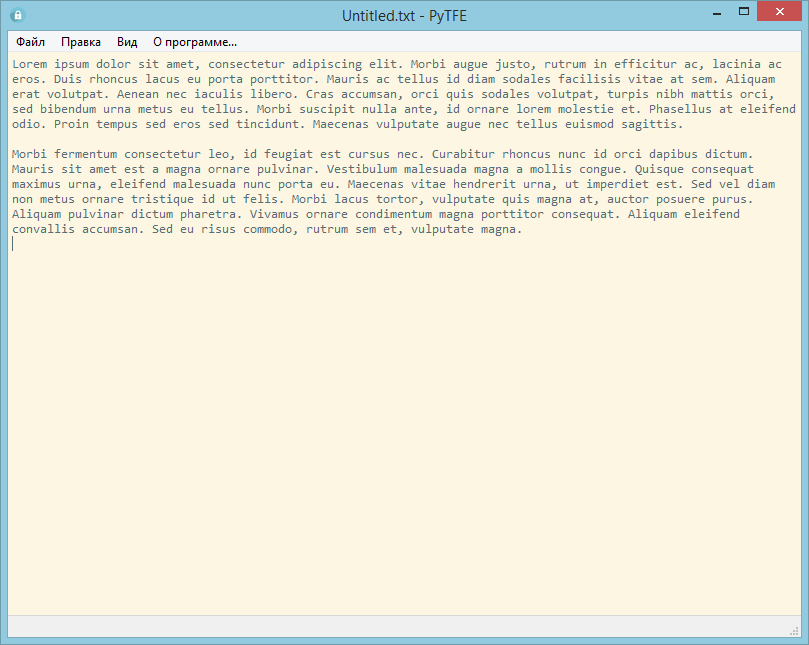
\includegraphics[scale=0.6]{./pics/te/app-main-window.png}
  \captionof{figure}{Вид главного окна программы}\label{fig:app-main-window}
  \vspace{3.5mm}
\end{minipage}

\noindent
\begin{minipage}{\linewidth}
  \vspace{3.5mm}
  \centering
  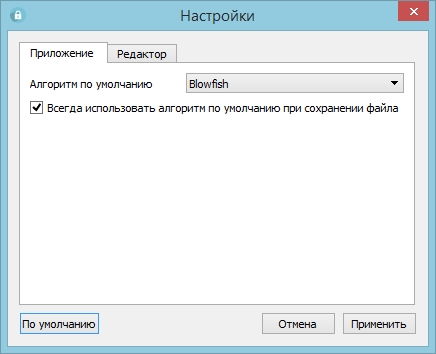
\includegraphics[scale=0.6]{./pics/te/app-settings-window-1.png}
  \captionof{figure}{Вид окна настроек: основные настройки}\label{fig:app-settings-window-1}
  \vspace{3.5mm}
\end{minipage}

\noindent
\begin{minipage}{\linewidth}
  \vspace{3.5mm}
  \centering
  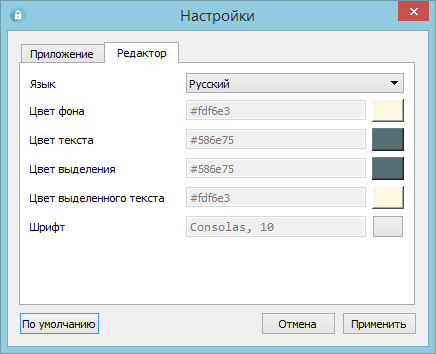
\includegraphics[scale=0.6]{./pics/te/app-settings-window-2.png}
  \captionof{figure}{Вид окна настроек: настройки редактора}\label{fig:app-settings-window-2}
  \vspace{3.5mm}
\end{minipage}

\subsection{Перевод приложения}

Библиотека Qt5 имеет средство для интернационализации (перевода) приложений.
С помощью утилиты \texttt{lupdate} создаются файлы локализаций,
которые содержат перевод строк в графическом интерфейсе в формате XML.
Редактирование файлов локализаций (перевод приложения)
осуществляется утилитой \texttt{linguist}. Утилита \texttt{lrelease} позволяет
``скомпилировать'' файлы локализаций для использования в готовом приложении.

В разработанной программе имеется поддержка
русского (рисунок \ref{fig:app-russian})
и английского (рисунок \ref{fig:app-english}) языка.

\noindent
\begin{minipage}{\linewidth}
  \vspace{3.5mm}
  \centering
  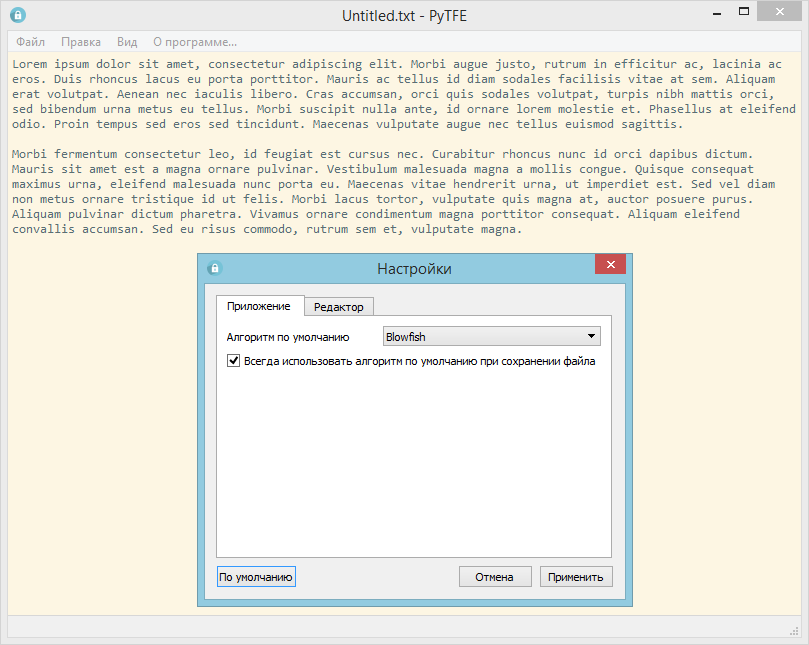
\includegraphics[scale=0.6]{./pics/te/app-russian.png}
  \captionof{figure}{Русский графический интерфейс}\label{fig:app-russian}
  \vspace{3.5mm}
\end{minipage}

\noindent
\begin{minipage}{\linewidth}
  \vspace{3.5mm}
  \centering
  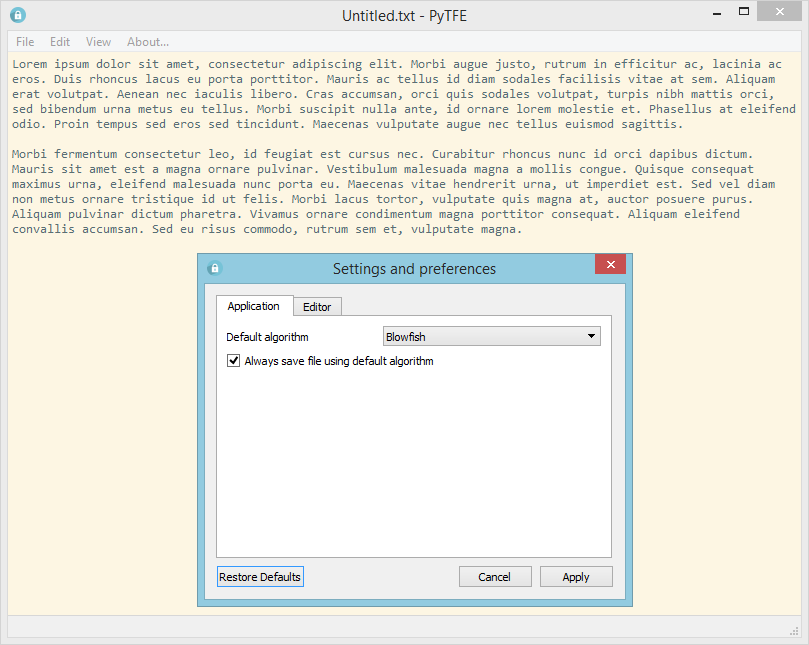
\includegraphics[scale=0.6]{./pics/te/app-english.png}
  \captionof{figure}{Английский графический интерфейс}\label{fig:app-english}
  \vspace{3.5mm}
\end{minipage}


% Заключение
% !TEX root = ../main.tex
\newpage
\ssection{Заключение}

При выполнении работы было спроектировано и реализовано программное средство,
позволяющее пользователям работать с зашифрованными текстовыми файлами.

К достоинствам разработанной программы можно отнести:
\begin{itemize}
  \item Простоту пользовательского интерфейса;
  \item Достаточный функционал;
  \item Наличие русского и английского переводов.
\end{itemize}

К недостаткам относятся:
\begin{itemize}
  \item Снижение скорости шифрования из-за частичного использования
  Python в модулях шифрования;
  \item Использование метода шифрования EBC;
\end{itemize}

Основываясь на результатах работы можно сделать следующие выводы:
\begin{itemize}
  \item Использование ассемблерного языка замедляет процесс написания
  программного кода и усложняет отладку программы.
  \item При использовании языка C упрощается процесс разработки и отладки
  программы в сравнении с языком ассемблера. Таким образом, язык C удобен
  для написания участков кода, от которых требуется высокая
  скорость выполнения.
  \item Использование интерпретируемого языка Python целесообразно для
  написания участков кода, от которых не требуется высокая скорость выполнения.
  Python значительно упрощает разработку и отладку программы в сравнении
  с языком C.
\end{itemize}


% Источники
% !TEX root = ../main.tex
\newpage
\renewcommand{\refname}{Список источников} % \bibname
%\bibliographystyle{gost780s} % ГОСТ 7.80
\begin{thebibliography}{9}
\addcontentsline{toc}{section}{\refname}

\bibitem{gnupg}
  Лозовюк А. GnuPG -- OpenSource шифрование и цифровые подписи.
  [Электронный ресурс]. -- Режим доступа: \\
  \verb'http://citforum.ru/security/cryptography/gnupg/', свободный.

\bibitem{python-docs}
  Документация по Python 3.4.3 [Электронный ресурс], 1990-2015. -- Режим доступа: \\
  \verb'https://docs.python.org/3.4/', свободный.

\bibitem{qt5-docs}
  Документация по Qt 5.5 [Электронный ресурс], 2015. -- Режим доступа: \\
  \verb'http://doc.qt.io/qt-5/', свободный.

\bibitem{panasenko}
  Панасенко С. П. Алгоритмы шифрования. Специальный справочник. --
  СПб.: БХВ-Петербург, 2009. -- 576 с.: ил.

\bibitem{feal-attack}
  Matsui M., Yamagishi A. A New Method for Known Plaintext Attack of
  FEAL Cipher. [Электронный ресурс], 1992. -- Режим доступа: \\
  \verb'http://link.springer.com/content/pdf/10.1007%2F3-540-47555-9_7.pdf'

\bibitem{blowfish}
  Schneier, B. Description of a New Variable-Length Key, 64-Bit Block Cipher (Blowfish)
  [Электронный ресурс]. -- Режим доступа: \\
  \verb'https://www.schneier.com/cryptography/archives/1994/09/description_of_a_new.html',
  свободный.

\end{thebibliography}


% FEAL-NX Specs:
%     http://info.isl.ntt.co.jp/crypt/eng/archive/dl/feal/call-3e.pdf
% Blowfish Specs:
%
% Blowfish encryption algorithm:
%     Bruce Schneier
%     https://www.schneier.com/cryptography/archives/1994/09/description_of_a_new.html
%
%
% Обзор GPG:
%     http://citforum.ru/security/cryptography/gnupg/


% Приложения
% !TEX root = ../main.tex
\newpage
\ssection{ПРИЛОЖЕНИЕ А}

\subsection*{Реализация FEAL-4 на языке C -- \texttt{feal4.c}}
\easycode{../prg/pytfe/src/algs/feal4/feal4.c}
\vspace{5mm}

\newpage
\subsection*{Реализация FEAL-4 на языке ассемблера -- feal4.asm}
\easycode{../prg/pytfe/src/algs/feal4/feal4.asm}
\vspace{5mm}

\newpage
\subsection*{Реализация Blowfish на языке C -- \texttt{blowfish.c}}
\easycode{../prg/pytfe/src/algs/blowfish/blowfish.c}
\vspace{5mm}

\newpage
\subsection*{Реализация Blowfish на языке ассемблера -- \texttt{blowfish.asm}}
\easycode{../prg/pytfe/src/algs/blowfish/blowfish.asm}
\vspace{5mm}

\newpage
\newpage
\ssection{ПРИЛОЖЕНИЕ Б}

\subsection*{Связка динамической библиотеки FEAL-4 с Python -- \texttt{feal4.py}}
\easycode{../prg/pytfe/src/app/mlibs/feal4.py}
\vspace{5mm}

\newpage
\subsection*{Связка динамической библиотеки Blowfish с Python -- \texttt{blowfish.py}}
\easycode{../prg/pytfe/src/app/mlibs/blowfish.py}
\vspace{5mm}

\newpage
\subsection*{Модуль для шифрования -- \texttt{tfe.py}}
\easycode{../prg/pytfe/src/app/mlibs/tfe.py}
\vspace{5mm}


\newpage
\ssection{ПРИЛОЖЕНИЕ В}
\subsection*{Начальные значения ключей и таблиц замены алгоритма Blowfish}
\easycode{../prg/pytfe/src/algs/blowfish/blowfishPS.c}
\vspace{5mm}


\end{document}
